\documentclass[a4paper,12pt,final]{article}
% Generic commands
\usepackage{draftcommands}

% Font encodings
\usepackage[T1]{fontenc}

% Sets margins
\usepackage[lmargin=1in,rmargin=1in,bmargin=1in,tmargin=.75in]{geometry}

% For hyperlinks, as usual
\usepackage{hyperref}

% The list of publications (with links)
\usepackage[backend=biber,maxcitenames=1,doi=true,url=true,sorting=ydnt,giveninits=true,defernumbers=true]{biblatex}
\addbibresource{cv.bib}

% Only use url if doi is not present
\DeclareSourcemap{
  \maps[datatype=bibtex]{
    \map[overwrite]{
      \step[fieldsource=doi, final]
      \step[fieldset=url, null]
      \step[fieldset=eprint, null]
    }  
  }
}

% Multiple language

% \providecommand{\kgdlang}{french}
\providecommand{\kgdlang}{english}
\usepackage[french,english,main=\kgdlang]{babel}
\usepackage{csquotes}
\usepackage{iflang}

\def\En#1{#1}
\def\Fr#1{}
\IfLanguageName{french}{%
 \def\En#1{}\def\Fr#1{#1}
 \usepackage[T1]{fontenc}
}{}

% Classification CNU 27

% Ouvrages
% Conférences invitées internationales
% Conférences invitées nationales

% Revues internationales avec comité de lecture
% Revues nationales avec comité de lecture
\def\publijournal{
    \En{Journals}%
    \Fr{Journaux Internationaux}%
    \ (peer-reviewed)}

% Chapitres de livre avec comité de lecture
% Direction d’ouvrages, de revues, actes
% Conférences internationales avec comité de lecture
% Conférences nationales avec comité de lecture
\def\publiconference{
    \En{International conferences}%
    \Fr{Conf\'erences Internationales}%
    \ (peer-reviewed)}

% Workshops/ateliers internationaux avec comité de lecture
% Workshops/ateliers nationaux avec comité de lecture
\def\publiworkshop{
    \En{Workshops}%
    \Fr{Workshops}}

\def\publiposter{
    \En{Posters}%
    \Fr{Posters}}

\def\publitalk{
    \En{Oral presentations}%
    \Fr{Pr\'esentations orales}}

% Séminaires invités
% Démonstrations
% Conférences sans comité de lecture
% Brevets, productions logicielles, mise à disposition de données.
\def\publisoftware{
    \En{Softwares and datasets}%
    \Fr{Logiciels, mise à disposition de données}}

% Autres (rapports, expertises, etc)
\def\publithesis{
  \En{Thesis}%
  \Fr{Th\`ese}}
  
\input{_bibliography_sections}

\newcommand\sectionedbibliography{
 \nocite{*}

 % More breathing room
 \emergencystretch=1em

 \foreach \subtype/\text in \publiclasses {
  \section*{\text}
  \printbibliography[heading=none, subtype=\subtype]
 }
}

% To draw the skill circles
\usepackage{tikz}
\usetikzlibrary{calc,fadings,shadings}

\tikzfading[name=fade out,inner color=transparent!0,outer color=transparent!100]
\newcommand{\skilldisk}[1]{%
 \def\sbcolor{red}
 \hspace{.5em}%
 \def\R{.15cm}%
 \begin{tikzpicture}[remember picture]%
  \pgfmathsetmacro\A{90-3.6*#1}
  \def\bgcolor{gray!40}
  \def\fgcolor{\sbcolor!50}
  
  \fill [white] (0,0) circle (\R);
  
  \shade[ball color = \bgcolor, opacity = 0.4] (0,0) circle (\R);
  \shade[ball color = \fgcolor, opacity = 0.8] (0,\R) arc (90:\A:\R) -- (0,0) -- cycle;
 \end{tikzpicture}%
}

% Main tabular layout
% \usepackage{booktabs} % Surprisingly un-used here
\usepackage{longtable} % Pagebreak-able tables
\usepackage{makecell} % Encapsulated tabular cell contents

\usepackage{url}

% The euro symbol
\usepackage{eurosym}

% Symbols in the contact section
\usepackage{fontawesome}

% To compute available rspace based on lspace
\usepackage{calc}

% Put pages number in footer
\usepackage{lastpage}
\usepackage{fancyhdr}

\def\fancysize{\small}

\fancyfoot[C]{\fancysize \thepage\ \En{of}\Fr{sur} \pageref*{LastPage}}
\fancyhead{}
 
\fancypagestyle{fancyfirst}{
 \fancyhead{}
 \fancyfoot[L]{\fancysize \En{Updated on} \today{}}
 \fancyfoot[C]{\fancysize \faRefresh \href{https://github.com/kgd-al/CV/raw/master/cv.pdf}{\En{Up-to date version}%
                                                                                           \Fr{Version \`a jour (Anglais)}}}
 \fancyfoot[R]{\fancysize \footnotesize Page \thepage\ \En{of}\Fr{sur} \pageref*{LastPage}}
}
\fancyfoot[C]{Page \thepage{} \En{of}\Fr{sur} \pageref*{LastPage}}

\renewcommand{\headrulewidth}{0pt}
\pagestyle{fancy}
\thispagestyle{fancyfirst}

% For (excessively) pretty underlining
\usepackage{contour}
\usepackage[normalem]{ulem}
\renewcommand{\ULdepth}{2pt}
\contourlength{0.8pt}
\newcommand{\prettyuline}[1]{%
 \uline{\phantom{#1}}%
 \llap{\contour{white}{#1}}%
}

% Helper for the mail links
\def\mailto#1{\small\href{mailto:#1}{\texttt{#1}}}

% Pdf meta-data
\En{\def\me{Kevin Godin-Dubois}}
\Fr{\def\me{K\'evin Godin-Dubois}}
\makeatletter
\hypersetup{
 pdfinfo={
  Author={\me},
  Title={\me{} - CV}
 }
}
\makeatother

% No indent
\setlength\parindent{0pt}

% =============================================================================
% Draft section

% To monitor file inclusion (in git)
\listfiles 

% Overfull hbox debugging
\overfullrule=1mm

% Prepare lengths
\newlength\lwidth
\setlength\lwidth{.2\textwidth}
\newlength\cwidth
\setlength\cwidth{\dimexpr2\tabcolsep}
\newlength\rwidth
\setlength\rwidth{\dimexpr\textwidth-\lwidth-\cwidth-.4pt}

% Local variables
\newlength\titlewidth
\newlength\titleoffset

\newenvironment{sect}[2][{\\*[0pt]}]{%
 \def\title{\Large\prettyuline{\texttt{\textbf{#2}}}}%
 \setlength{\titlewidth}{\widthof{\title}}%
 \setlength{\titleoffset}{\maxof{0pt}{\lwidth-\titlewidth*\real{0.5}}}%
%  lwidth: \the\lwidth \\
%  title width: \the\titlewidth\\
%  title offset: \the\titleoffset \\
%  
 \begin{longtable}{@{}c|c@{}}%\\\\[-.75cm]
  \multicolumn{2}{l}{\hspace{\titleoffset}\title}\vspace{-2.9pt}\\*#1%\\[-10pt]
}{%
 \end{longtable}%
}%

\def\dbgrule{}
% \def\dbgrule{\hline}
\newcommand{\itm}[3]{%
\dbgrule%
 \makecell[t{p{\lwidth}}]{%
  \raggedleft%
  \ifx\hfuzz#1\hfuzz\else%
   \textbf{#1}%
   \ifx\hfuzz#2\hfuzz\else\\\fi%
  \fi%
  #2%
 } & \makecell[t{p{\rwidth}}]{#3} \\
\dbgrule
}

\def\di{$\bullet$\ }
\def\dii{\hspace{1.5em} $\circ$\ }
\renewcommand{\labelitemi}{\di}
\renewcommand{\labelitemii}{\dii}

% ========================================
\def\UnivUPSShort{%
  \En{Toulouse III University}%
  \Fr{Universit\'e Toulouse III Paul Sabatier}%
}
\def\UnivUPS{\UnivUPSShort, France}
% ========================================
\def\UnivCapitoleShort{%
  \En{Toulouse I University}%
  \Fr{Universit\'e Toulouse I Capitole}%
}
\def\UnivCapitole{\UnivCapitoleShort, France}
% ========================================
\def\UnivVUShort{Vrije Universiteit Amsterdam}
\def\UnivVU{\UnivVUShort, The Netherlands}
% ========================================

% ========================================
% Format skills
\newcommand{\formatskill}[2]{\skilldisk{#2} \small#1}
\def\cols(#1)#2{%
 \itm{}{#1}{%
  \foreach \p/\l in {#2} {%
   \begin{minipage}{.32\rwidth}\formatskill{\l}{\p}\end{minipage}%
  }%
 }%
}

% ========================================

% \usepackage{showframe}

% Display width repartition
\def\dbgshowwidths{
 \tikz [remember picture, overlay]
  \node at (current page.north) [anchor=north]
   {{\color{red}\rule{\lwidth}{1mm}}{\color{green}\rule{\cwidth}{1mm}}{\color{blue}\rule{\rwidth}{1mm}}};
}
\reversemarginpar
\def\ok{}%\marginpar{\tikz\fill[green,draw=green!50!black,scale=1](0,.35) -- (.25,0) -- (1,.7) -- (.25,.15) -- cycle;}}

% ========================================

\graphicspath{{../resources/cv/}}

% =============================================================================
% Contents
% =============================================================================
\begin{document}
% \dbgshowwidths%
\vspace{-1\baselineskip}
\ok
\begin{sect}{\Huge Dr.\enspace\me}
 \itm{Contact}{}{%
  \centering\begin{tabular}[t]{c@{ }m{.35\textwidth}c@{ }m{.3\textwidth}}
   \faEnvelopeO & \mailto{k.j.m.godin-dubois@vu.nl}
     & \faGithub & \href{https://github.com/kgd-al}{kgd-al@github.com} \\                       
   \faHome & \UnivVUShort
     & \faVimeo & \href{https://vimeo.com/godinduboisalife}{godinduboisalife} \\
           & de Boelelaan 1081a, 1081HV
     & 
\includegraphics{misc/academicons_gscholar}
       & \href{https://scholar.google.com/citations?user=8k1MH20AAAAJ}{Google Scholar} \\
           & Amsterdam, The Netherlands
     & 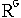
\includegraphics{misc/academicons_rgate}
       & \href{https://www.researchgate.net/profile/Kevin-Godin-Dubois}{ResearchGate}
  \end{tabular}
 }
 \\[-.5em]
 \itm{Position}{}{Researcher in Evolutionary Robotics (since November 2022)}
\end{sect}

\ok
\begin{sect}{Highlights}
 \itm{\En{Research}\Fr{Recherche}}{}{%
  \large\emph{\En{Artificial Life: Cognition, Interaction \& Language}}
 }
 \\[-.5em]
 
 \itm{}{\En{Main fields}\\}{%
  \hfill
  \foreach \i/\lEn/\lFr in
   {ann_vfmri_colored/Artificial Neural Networks/??,
    phylogenetics_colored/Species Dynamics/Dynamiques d'esp\`eces,
    splinoids_morphos/Morphogenetic Engineering/Morphogenetic Engineering} {
   \begin{minipage}[t]{.22\textwidth}
    \centering
    \includegraphics[width=\textwidth]{\i} \\
    \small\En{\lEn}\Fr{\lFr}
   \end{minipage}
   \hfill
  } 
 }
 \\[-.25em]
 
 \itm{}{\En{Publications}}{%
  1 journal article (\emph{Artificial Life}) \\
  4 international conference articles (\emph{ALife, IEEE ALife, EvoAPP})\\
  4 international workshops short papers (\emph{ALife, ECAL})%\\
%   1 poster (\emph{ALife})
 }
 \\[.5em]
 
 \itm{Positions}{}{}
 \\[-.5em]
 
 \itm{{\normalfont Postdoctoral}}{\emph{2022 - Present}}{%
  Computer Science / Evolutionary Robotics \\
  \emph{``NeuroEvolution and Reinforcement Learning for Embodied Robots''} \\
  Computational Intelligence Group - \UnivVU \\
  \begin{tabular}{@{}r@{ }l@{}}
   Supervisor:   & Dr. K. Miras \hfill(\mailto{k.dasilvamirasdearaujo@vu.nl}) \\
  Collaborators: & Dr. A. Kononova \hfill(\mailto{a.kononova@liacs.leidenuniv.nl}) \\
                 & Dr. D. Mocanu \hfill(\mailto{d.c.mocanu@utwente.nl}) \\
  \end{tabular}
 }
 \\[.5em]
 
 \itm{{\normalfont Postdoctoral}}{\emph{2020 - 2022}}{%
  Computer Science / Artificial Intelligence \\
  \emph{``Emergent cognitive architectures in virtual embodied robots''} \\
  REVA Team, IRIT - \UnivCapitole \\
  Supervisors: Pr. Y. Duthen \hfill(\mailto{yves.duthen@irit.fr}) \\
  \phantom{Supervisors: }Pr. S. Cussat-Blanc \hfill(\mailto{sylvain.cussat-blanc@irit.fr})
 }
 \\[.5em]
 
 \itm{\normalfont PhD}{\emph{2016-2020}}{%
  Computer Science / Artificial Life \\
  \emph{``Environment-driven speciation: long term interactions in artificial plant communities''} \\
  REVA Team, IRIT - \UnivCapitole \\
  Supervisors: Pr. Y. Duthen \hfill(\mailto{yves.duthen@irit.fr}) \\
  \phantom{Supervisors: }Pr. S. Cussat-Blanc \hfill(\mailto{sylvain.cussat-blanc@irit.fr})
 }
%  \\[.5em]
 \newpage
 
 \itm{\En{Teaching}}{}{6 years (507 hours)}
 \\[-.5em]
 
 \itm{}{Computer\\ Science}{
  Learning Machines Master 2 Projects \\
  Programming languages: Python, C, R \\
  Algorithms, Data Structures, Information theory \\
  Programming projects
 }
 \\[-.5em]
 
 \itm{}{Generalists}{
  Data Science tools and languages \\
  Database modeling, SQL
 }
 \\[.25em]
 
 \itm{Skills}{}{}
 \itm{}{Programming}{
  Fluent: \cpp, Bash, Python, \LaTeX \\
  Working Knowledge: C, Java, R, VB, VBA
 }\\[-.75em]
 \itm{}{Technical}{Evolutionary Algorithms, Machine Learning, Multi-Agents Systems, High-Performance Computing}
 \\[-.75em]
 \itm{}{Languages}{French (Mother tongue), English (Fluent - 980/990 at the TOEIC)}
\end{sect}
% \newpage

\newcommand{\ritm}[5]{%
 \itm{}{%
  \begin{minipage}[t]{\lwidth}%
   \vspace{0pt}%
   \raggedleft
   \includegraphics[width=\textwidth, height=4em, keepaspectratio]{#1}%
  \end{minipage}%
 }{%
  \begin{minipage}[t]{\rwidth}%
   \vspace{0pt}\small%
   \cite{#4} \textsc{\En{#2}\Fr{#3}} \\%
   #5%
  \end{minipage}%
 }
}
\newcommand{\sref}[3][Software]{\textbf{#1:} \href{#2}{#3}}
\begin{sect}{Research}
 \itm{Synopsis}{}{%
  \small My main interests revolve around the production of autonomous artificial life forms: from the autonomous design of efficient morphologies to the emergence of high-level control schemes and the evolutionary constraints that favor both.
  The former and latter were investigated throughout my thesis whereas my more recent work deals with Artificial Neural Networks (ANN), with a special focus on the transition from communication to language and its neural implementation.
%   After a PhD thesis focused on artificial plant-like lifeforms and their dynamics at the evolutionary scale, I am returning to my core interest: artificial cognition.
%   More specifically, I am investigating the mechanisms by which high-level forms of interaction (e.g. vocal communication) can be built upon low-level inputs/outputs thanks to (a)biotic constraints.
 }
 \\
 
 \itm{Artificial Neural Networks}{}{
  Studying the emergence of various ``cognitive'' capabilities in virtual robots, controlled by a spontaneously differentiated neural network, in response to biologically plausible stimuli.
 }
 \ritm{ann_vfmri_colored}{Virtual fMRI}{IRMf virtuelle}{GodinDubois2021a,GodinDubois2023a}{
  Extracting stimulus-specific regions of an ANN by applying a virtual equivalent to functional Magnetic Resonance Imaging (fMRI) and building high-level cognitive maps. \\
  \sref{https://github.com/kgd-al/ES-HyperNEAT}{ES-HyperNEAT} (Custom implementation)
 }
%  \ritm{mew}{Species dynamics}{Dynamiques d'esp\`eces}{GodinDubois2019b}{}
 \ritm{communication}{Communication}{Communication}{GodinDubois2021b,GodinDubois2022a}{
  Exploring the mechanisms leading to emergent communication, how it becomes structured and its neural implementation.
 }
 \\[.5em]

 \itm{Species Dynamics}{}{
  Promoting complex evolutionary trajectories and extracting species-level information from individual reproductions. 
 }
 \ritm{phylogenetics_colored}{Phylogenetics}{Phylog\'en\'etiques}{GodinDubois2018u,GodinDubois2019c}{
  Automatically transforming genealogic trees into phylogenetic abstraction to access the emergent species-level dynamics. \\
  \sref{https://github.com/kgd-al/APOGeT}{APOGeT}{(Automated Phylogeny Over Geological Timescales)}
 }
 \ritm{species_dynamics}{Speciation}{Dynamiques d'esp\`eces}{GodinDubois2019b}{
  Application of a bio-inspired reproduction operator (Bail-Out Crossover) capable of spontaneously generating species barriers thereby allowing for emergent speciation.
 }
 \ritm{edens_algo}{Evolutionary algorithms}{Algorithmes \'evolutionnaires}{GodinDubois2020a,GodinDuboisThesis}{
  Introduced a novel paradigm, EDEnS (Environment-Driven Evolutionary Selection), relying on the indirect controlling of whole populations' evolutionary trajectories through an evolvable environmental controller.
 }
 \\[.5em]

 \itm{Morphogenetic Engineering}{}{
  Concerned with the development of functional morphology in response to environmental constraints and evolutionary pressures.
 }
 \ritm{mew}{Developmental morphologies}{Morphologies d\'evelopementales}{Dubois2017,GodinDubois2020a,GodinDubois2019a,GodinDubois2018u}{
  Production of mature, functional virtual plants from a single cell/structure using various genetic encodings (rules-based, L-Systems, Graphtals) in response to environmental constraints.
 }
 \ritm{splinoid_morpho}{Virtual robots}{Robot virtuels}{GodinDubois2023a} {
  Use of genetically parameterized cubic b\'ezier curves to control both static and mobile structures on the perimeter of virtual circular robots. \\
  \sref{https://github.com/kgd-al/Splinoids}{Splinoids} \hfill 
  \sref[Videos]{https://vimeo.com/showcase/9613894}{on Vimeo} \hfill\null
 }
 \\[.5em]

 \itm{Expertise}{}{}
 \\[-.5em]
 \itm{}{Evolutionary Algorithms}{
  \di Environment-Driven Evolutionary Selection (EDEnS) \\
  \di Multi-objective Optimisation \\
  \di High Performance Computing (HPC), Co-evolution, Novelty
 }
 \\[-.5em]
 \itm{}{Machine Learning}{
  \di Artificial Neural Networks (ANN, CNN, RNN) \\
  \di Composite Pattern-Producing Networks (CPPN) \\
  \di Cartesian Genetic Programming (CGP) \\
  \di Genetic Regulatory Networks (GRN) \\
  \di Hidden Markov Models (HMM) \\
  \di Stable baselines 3
 }
%  \\[-.5em]
\end{sect}
% \newpage

\def\ritm#1{\hfill\emph{#1}}
\def\teachings{\En{Teachings}\Fr{Enseignements}}
\ok
\begin{sect}{\teachings}
%  \itm{}{}{Academic title and current position}

 \itm{\En{M2 Projects}\Fr{Projets M2}}{2023}{
  \UnivVUShort \\
  \di Learning Machines \ritm{15h} \\
  \di Master/Bachelor thesis supervision \\
 }
 \\[-.5em]

 \itm{\En{Course management}\Fr{Responsable d'UE}}{2021-2022}{
  \UnivCapitoleShort{} \& \UnivUPS \\  
  \di Computer Science projects \ritm{72h} \\
  {\small\emph{Multi-Agent Systems, Complex Systems, Simulation}} \\
  \di R programming \ritm{67.5h} \\
  {\small\emph{English lectures}} \\
  \di Information theory \ritm{22.5h} \\
  \di Servers and contents \ritm{18.75h} \\
 }
 \\[-.5em]
 
 \itm{\En{Teaching fellow}\Fr{Charg\'e de TD}}{2017-2021}{
  \UnivCapitoleShort{} \& \UnivUPS \\
  \di Statistical software (R \& Python) \ritm{36h} \\
  \di Algorithms \ritm{60h} \\
  \di Excel \& VBA \ritm{60h} \\
  \di Modeling in databases \ritm{21h} \\
 }
 \\[-.5em]
 
 \itm{\En{Practical work supervisor}\Fr{Charg\'e de TP}}{2016-2021}{
  \UnivUPS \\
  \di \En{Software projects}\Fr{Projet Logiciel} \ritm{69.2h} \\
  \di \En{Data structures}\Fr{Structure de donn\'ees} \ritm{18.8h} \\
  \di \En{C Programming}\Fr{Programmation C} \ritm{36h} \\
  \di Python \ritm{8h}
 }
\end{sect}

\begin{sect}{Outreach}
 \itm{Reviewer}{2023}{
  \di Symposium on Artificial Life program comitee member \\
  \di Journal of Open Source Software reviewer
 }\\
 \itm{EduMix Aspi-Friendly}{2021}{
  Initiated a project for the self-monitoring of well-being in students with autistic disorders alongside a heterogeneous team of neuro-(a)typical and various profiles (faculty, designers, developers ...).
 }
\end{sect}

\def\internship{\En{Internship}\Fr{Stage}s}
\def\months{\En{months}\Fr{mois}}
\ok
\begin{sect}{\internship}
 \itm{Morphogenetic Engineering}{2016 (6 \months)}{%
  \En{Toulouse Research Institute on Computer Science (IRIT)}%
  \Fr{Institut de Recherche en Informatique de Toulouse (IRIT)}%
    , France \\%
  \emph{%
    \En{``Rule-based artificial embryogenesis in a complex 3D environment''}%
    \Fr{``Embryogen\`ese artificielle dans un environnement 3D complexe''}%
  } \\%
  {\small%
    \En{Deployed rule-based genomes on the MecaCell platform to study artificial plant growth and cell specialization.}%
    \Fr{D\'eploiement de g\'enomes \`a base de r\`egles sur la plateforme MecaCell pour \'etudier la croissance de plantes et la sp\'ecialisation cellulaire.}%
  } \\
  \textbf{Contact:} Pr. Y. Duthen (\mailto{yves.duthen@irit.fr})
 }
 \\
 
 \itm{Machine Learning}{2015 (3 \months)}{
  IRIT, \emph{%
    \En{``Comparison of different evolutionary approaches, an application to the GECCO 2015 challenge''}%
    \Fr{``Comparaison d'approches \'evolutionnaires, une application au challenge GECCO 2015''}%
  } \\
  {\small%
    \En{Performed a performance comparison (accuracy, efficiency) between Artificial Neural and Genetic Regulatory Networks on the 2015 GECCO temperature prediction challenge data.}%
    \Fr{\'Etude sur les diff\'erences de performance entre R\'eseaux de Neurones Artificiels et R\'eseaux de R\'egulation G\'en\'etiques sur des donn\'ees de pr\'ediction de temp\'erature.}%
  } \\
  \textbf{Contact:} Pr. H. Luga (\mailto{herve.luga@irit.fr})
 }
 \\
 
 \itm{Machine Learning}{2014 (2 \months)}{
  IRIT, \emph{%
    \En{``An architecture for automated bird discrimination''}%
    \Fr{``Architecture pour la discrimination automatique d'oiseaux''}%
  } \\
  {\small%
    \En{Applied Hidden Markov Models to the BirdClef2014 challenge on the identification of specific bird species in a corpus of thousands of recordings.}%
    \Fr{Application de Mod\`eles de Markov Cach\'es au challenge BirdClef2014 pour l'identification d'esp\`eces d'oiseaux dans un large corpus.}%
  } \\
  \textbf{Contact:} Pr. J. Farinas (\mailto{jerome.farinas@irit.fr})
 }
\end{sect}

\newpage
\ok
\begin{sect}{\En{Education}\Fr{\'Education}}
 \itm{\En{PhD}\Fr{Doctorat}}{2016 - 2020}{%
  \UnivCapitole
  \\
  Defended the 15th of July 2020
  \\
  \En{Thesis title: \emph{``Environment-driven speciation: long term interactions in artificial plant communities''}}
  \Fr{Th\`ese: \emph{``Sp\'eciation guid\'ee par l'environnement: interactions \`a long terme de communaut\'es de plantes artificielles''}}
  \\
  {\small%
    \En{Investigated how complexification of artificial creatures could be further enhanced through the indirect control provided by a co-evolved, highly dynamical environment.}%
    \Fr{\'Etude sur la mani\`ere dont la complexification de cr\'eatures artificielles pourrait \^etre am\'elior\'ee gr\^ace au contr\^ole indirect exerc\'e par un environnement hautement dynamique et conjointement \'evolu\'e.}%
  } \\
  \textbf{Rapporteurs:} Pr. P. Collet \& DoR. F. Vico \\
  \textbf{Contact:} Pr. Y. Duthen (\mailto{yves.duthen@irit.fr})
 }
 \\
   
 \itm{Master}{2014 - 2016}{
  \UnivUPS{} (\emph{with honours})
  \\
  {\small%
    \En{Artificial Intelligence: mathematical \& symbolic models, training methods}%
    \Fr{Intelligence Artificielle: mod\`eles math\'ematiques et symboliques, m\'ethodes d'entra\^inement}
  }
 }
 \\
 
 \itm{\En{Bachelor}\Fr{Licence}}{2011 - 2014}{
  \UnivUPSShort{} (\emph{with distinction})
  \\
  {\small%
    \En{Computer Science: networks, programming, systems, mathematics}%
    \Fr{Informatique: r\'eseaux, programmation, syst\`emes, math\'ematiques}
  }
 }
\end{sect}
\ok
\begin{sect}{\En{Scholarships and Fellowships}%
             \Fr{Bourses}}
             
 \itm{2023-2026}{$\sim$ 200K \euro}
     {\En{Postdoctoral funding from the Hybrid Intelligence consortium (Netherlands)}%
      \Fr{Financement post-doctoral du consortium Hybrid Intelligence (Pays-bas)}}
 \\

 \itm{2016-2019}{70K \euro}
     {\En{PhD Fellowship from the French Minister of Higher Education and Research (MESR)}%
      \Fr{Bourse doctorale du Minist\`ere de l'Enseignement Sup\'erieur et de la Recherche}}
 \\
 
 \itm{2015}{10K \euro}
     {\En{Master Scholarship from the International Mathematics and Computer Science Center (LabEx CIMI, Toulouse)}%
      \Fr{Bourse de master du Centre International de Math\'ematiques et Informatique (Labex CIMI, Toulouse)}}
 \\
     
 \itm{2014-2015}{3K6 \euro}
     {\En{Merit Scholarship from the Regional Student Welfare Office (CROUS, Toulouse)}%
      \Fr{Bourses de m\'erite (CROUS, Toulouse)}}
\end{sect}
% \newpage

% ========================================

% **Manual** layout alteration
% \Fr{\vspace{2\baselineskip}}

\ok
\small
\renewcommand*{\bibfont}{\normalfont\small}
\begin{sect}[]{\En{Research Output}%
               \Fr{Production Scientifique}}
 \multicolumn{1}{m{\lwidth}}{} & \multicolumn{1}{m{\rwidth-11.6pt}}{} \\*
\end{sect}%
\vspace{-\baselineskip}
\nocite{*}%
% \textbf{\publipending}
% \printbibliography[heading=none, type=unpublished]
\textbf{\publijournal}
\printbibliography[heading=none, subtype=journal]
% \En{\newpage}
\textbf{\publiconference}
\printbibliography[heading=none, subtype=conference]
\textbf{\publiworkshop}
\printbibliography[heading=none, subtype=workshop]
\textbf{\publiposter}
\printbibliography[heading=none, subtype=poster]
\textbf{\publioral}
\printbibliography[heading=none, subtype=talk]
\textbf{\publithesis}
\printbibliography[heading=none, type=thesis]

\end{document}
